\section{Coplanar waveguide resonators}

\dropcap{S}{ince} a dissertation is a substantial document, it is convenient to break it up into smaller pieces. In this template we therefore give every chapter its own file. The chapters (and appendices) are gathered together in \texttt{dissertation.tex}, which is the master file describing the overall structure of the document. \texttt{dissertation.tex} starts with the line

\subsection{Transmission line theory}

\subsection{Lumped-element circuit model}
\begin{figure}
	\centering
	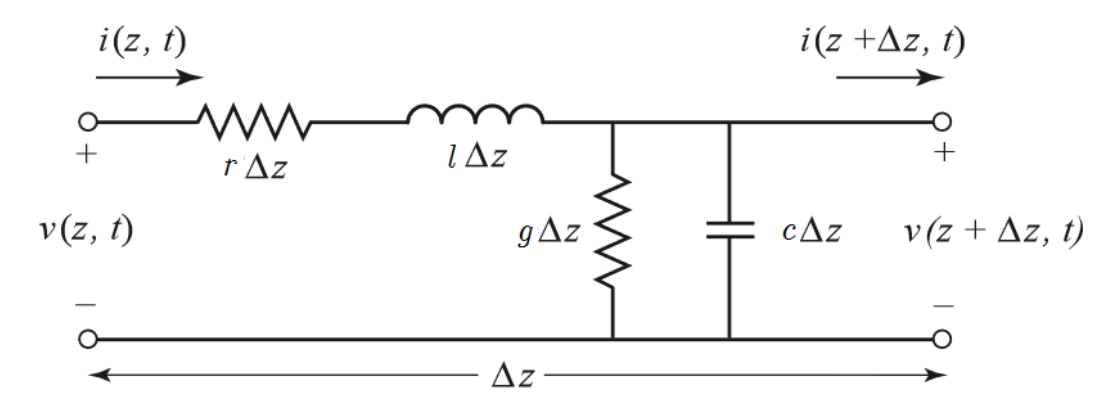
\includegraphics[width=0.4\linewidth]{chapter-theory/figs-RF/TL_lumped}
	\caption{Lumped element model of an infinitesimal short piece of a transmission line.}
	\label{fig:tllumped}
\end{figure}
We can model a transmission line, on which electromagnetic waves travel, by thinking of the EM waves as voltages and currents propagating along a distributed element circuit. This circuit can be split into infinitesimal small elements, depicted in figure \ref{fig:tllumped}, with series resistors and inductors, and parallel conductances and capacitances. In the following, we apply Kirchoff's laws to the circuit. The voltage and current of this network are given by
\begin{align}
v(z,t) - r\Delta z i(z,t) - l\Delta z\frac{\partial i(z,t)}{\partial t}-v(z+\Delta z,t) &=0 \\%
i(z,t) - g\Delta z v(z+\Delta z, t) - c\Delta z\frac{\partial v(z+\Delta z,t)}{\partial t} - i(z+\Delta z,t) &=0
\end{align}
For the limit $\Delta z\rightarrow0$ these equations transform into 
\begin{align}
\frac{\partial v(z,t)}{\partial t} &= -ri(z,t)-l\frac{\partial i(z,t)}{\partial t} \\%
\frac{\partial i(z,t)}{\partial t} &= -gi(z,t)-c\frac{\partial v(z,t)}{\partial t}
\end{align}
Rewriting these equations for sinusoidal steady-state conditions and cosine-based phasors, i.e. $x(z,t) \rightarrow X(z)e^{i\omega t}$ results in the \textit{Telegrapher equations:}
\begin{align}
\frac{d^2V}{dz^2} = \gamma^2V(z) \hspace{2cm} \frac{d^2I}{dz^2} = \gamma^2I(z)
\label{eq:telegraph}
\end{align}
with the complex propagation constant
\begin{equation}
\gamma = \alpha + j\beta =\sqrt{(R+j\omega L)(G+j\omega C)}
\label{eq:gamma}
\end{equation}
where $\alpha$ is the attenuation constant and we defined $j=-i$ to avoid confusion with the current. The solutions to these are traveling waves of the form
\begin{equation}
V(z) = V_0^+e^{-\gamma z} + V_0^-e^{\gamma z} \hspace{2cm} I(z) = I_0^+e^{-\gamma z} + I_0^-e^{\gamma z}
\label{eq:telegraph:solution}
\end{equation}
Plugging these solutions into the telegrapher equations, we get for the current on the line $I(z)=\gamma/(R+j\omega L) * V(z)$. We can immediately see that the characteristic impedance of our transmission line is given by
\begin{align}
Z_0 \equiv \frac{V_0^+}{I_0^+}\equiv \frac{V_0^-}{I_0^-}= \frac{R+j\omega L}{\gamma} = \sqrt{\frac{R+j\omega L}{G + j\omega C}}
\end{align}
Converting this result back to the time-domain results in the following form of our voltage on the line:

\begin{align}
v(z,t) = \abs{V_0^+}\cos(\omega t-\beta z+\phi^+)e^{-\alpha z} + \abs{V_0^-}\cos(\omega t+\beta z+\phi^-)e^{\alpha z}
\end{align}

where $\phi^{\pm}$ is the phase angle of the complex voltage $V_0^{\pm}$. Hence it is clear that the wavelength on the line is $\lambda=2\pi/\beta$, and the phase velocity $v_p=\omega/\beta=\lambda f$.
\subsection{The lossless line}
In general, the propagation constant of electromagnetic waves on a transmission line is given by the propagation constant in equation \ref{eq:gamma}. For the lossless case $R=0$ and $G=0$ and the resulting propagation constant
\begin{align}
\gamma_\mathrm{lossless} &= j\omega\sqrt{LC} \\%
&\rightarrow \alpha=0, \; \beta=\omega\sqrt{LC}
\end{align}
For this case, we have no attenuation ($\alpha=0$) and the line impedance $Z_0=\sqrt{L/C}$ is real. The wavelength and frequency are then simply given by
\begin{equation}
\lambda = \frac{2\pi}{\beta} = \frac{2\pi}{\sqrt{LC}} \hspace{2cm} v_p=\frac{\omega}{\beta}=\frac{1}{\sqrt{LC}}
\end{equation}

\subsection{The terminated lossless transmission line}
\begin{figure}
	\centering
	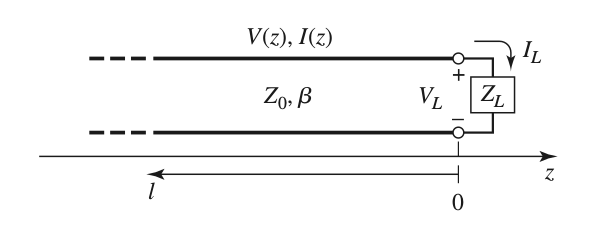
\includegraphics[width=0.4\linewidth]{chapter-theory/figs-RF/pozar_terminated_lossless}
	\caption{Sketch of a lossless transmission line terminated in a load impedance $Z_L$.}
	\label{fig:pozarterminatedlossless}
\end{figure}
Let us assume a terminated lossless line as depicted in Fig. \ref{fig:pozarterminatedlossless}. An incident Voltage wave $V_0^+ e^{-j\beta z}$ propagates from $z<0$ along the line to the right. $V/I$ of this line is $Z_0$. However, as the wave hits the termination, $Z_L \neq Z_0$, and a reflected wave is emitted to account for the impedance mismatch. Using eq. \ref{eq:telegraph:solution}, the resulting impedance at $z=0$ is 
\begin{align}
Z_L=\frac{V(0)}{I(0)}=Z_0\frac{V_0^++V_0^-}{V_0^+-V_0^-} \hspace{1cm} \rightarrow V_0^-=\Gamma Z_0 \\%
\Gamma = \frac{Z_L-Z_0}{Z_L+Z_0}
\end{align} 
where we defined $\Gamma$ as the voltage reflection coefficient.

\section{Coplanar waveguides}
To confine and guide electromagnetic waves on chips, we make use of coplanar waveguides. These consist of thin metal film of thickness $t$ on a dielectric substrate (thickness $H$). the metal film is patterned into a center conductor of width $w$ and is separated by the ground planes by a distance $s$ (see Fig. \ref{fig:cpw-coplanar-waveguide}). The characteristic impedance of such a CPW is given by
\begin{equation}
Z_0 = \sqrt{\frac{L'}{C'}}
\end{equation}
The electromagnetic waves in such a line are traveling with the wave velocity \begin{equation}
v=\frac{1}{\sqrt{L'C'}}=\frac{c_\mathrm{vac}}{\sqrt{\epsilon_\mathrm{eff}}}.
\end{equation}
If we assume a very thin film with large gaps, i.e. $t \ll s \ll H \rightarrow \infty$, and by defining the effective dielectric constant $\epsilon_\mathrm{eff} = \frac{1+\epsilon_r}{2}$, the transmission line parameters can all be reduced to the following expressions:
\begin{align}
C' &= 2\epsilon_0(\epsilon_r+1)\frac{K(K_0)}{K(k'_0)} \\%
L' &= \frac{\mu_0}{4}\frac{K(k'_0)}{K(k_0)} \\%
Z_0 &= \frac{c\mu_0}{\sqrt{8(\epsilon_r+1)}}\frac{K(k'_0)}{K(k_0)}\approx \frac{30\pi}{\sqrt{(\epsilon_r+1)/2}}\frac{K(k'_0)}{K(k_0)} \\%
v &= \frac{c}{\sqrt{(\epsilon_r+1)/2}}
\end{align}
\begin{figure}
	\centering
	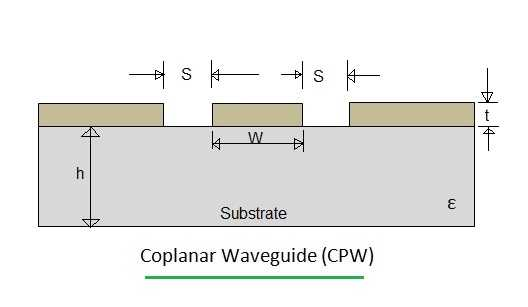
\includegraphics[width=0.3\linewidth]{chapter-theory/figs-RF/CPW-Coplanar-Waveguide.jpg}
	\caption{Cross section of a coplanar waveguide on a dielectric substrate.}
	\label{fig:cpw-coplanar-waveguide}
\end{figure}
where $K(q) = \frac{\pi}{2}\sum_{n=0}^{\infty}\left(\frac{(2n-1)!!}{(2n)!!}\right)^2 q^{2n}$ is the complete elliptic integral of the first kind, and
\begin{align}
k_0 = \frac{w}{w+2s} \hspace{2cm} k'_0 = \sqrt{1-k_0^2}.
\end{align}
Thus, it is obvious that all line parameters depend only on geometric factors, primarily on the ratio of center conductor width $w$ to gap separation $s$.


\section{Kinetic inductance}
For highly disordered superconductors, such as MoRe or NbTiN, there is an additional effect to be taken into account when analysing or designing a circuit: The so-called \textit{kinetic inductance} $L_k$. It arises naturally from the Drude model, when considering electron relaxation times comparable to the excitation frequency. This then leads to an additional inductance term from the kinetic energy of the electrons that are "lagging behind" the excitation signal. For a superconducting wire with length $l$ and crossection $A$, it is given by
\begin{eqnarray}
L_k = \frac{m}{2n_s e^2}\frac{l}{A}
\end{eqnarray}
with $n_s$ the Cooper pair density. For a CPW, $L_k$ reads
\begin{eqnarray}
L_k = g L_s = g\mu_0\lambda_m\coth\left(\frac{t}{\lambda_m}\right)
\end{eqnarray}
where $L_s$ denotes the surface inductance, $t$ the film thickness, $g=g(S,W,t)$ the geometry factor of the CPW, $\Delta_0\approx1.764\,k_BT_c$ the superconducting gap at \SI{0}{K} and $\lambda_m$ the London penetration depth at $T\rightarrow0$ as
\begin{eqnarray}
\lambda_m=\sqrt{\frac{\hbar\rho}{\pi\mu_0\Delta_0}}\approx\SI{105}{(nm)}\cdot\sqrt{\frac{\rho\si{\,(\micro\ohm\,\centi\metre)}}{T_c \si{\,(K)}}}
\end{eqnarray}
This length changes as a function of temperature according to
\begin{eqnarray}
\lambda_m(T) = \frac{\lambda_m(0)}{\sqrt{1-\left(\frac{T}{T_c}\right)^4}}
\end{eqnarray}

\subsection{Current bias cavities, or series RLC circuit capacitively coupled to one side of a transmission line}
\begin{figure}[!h]
	\centering
	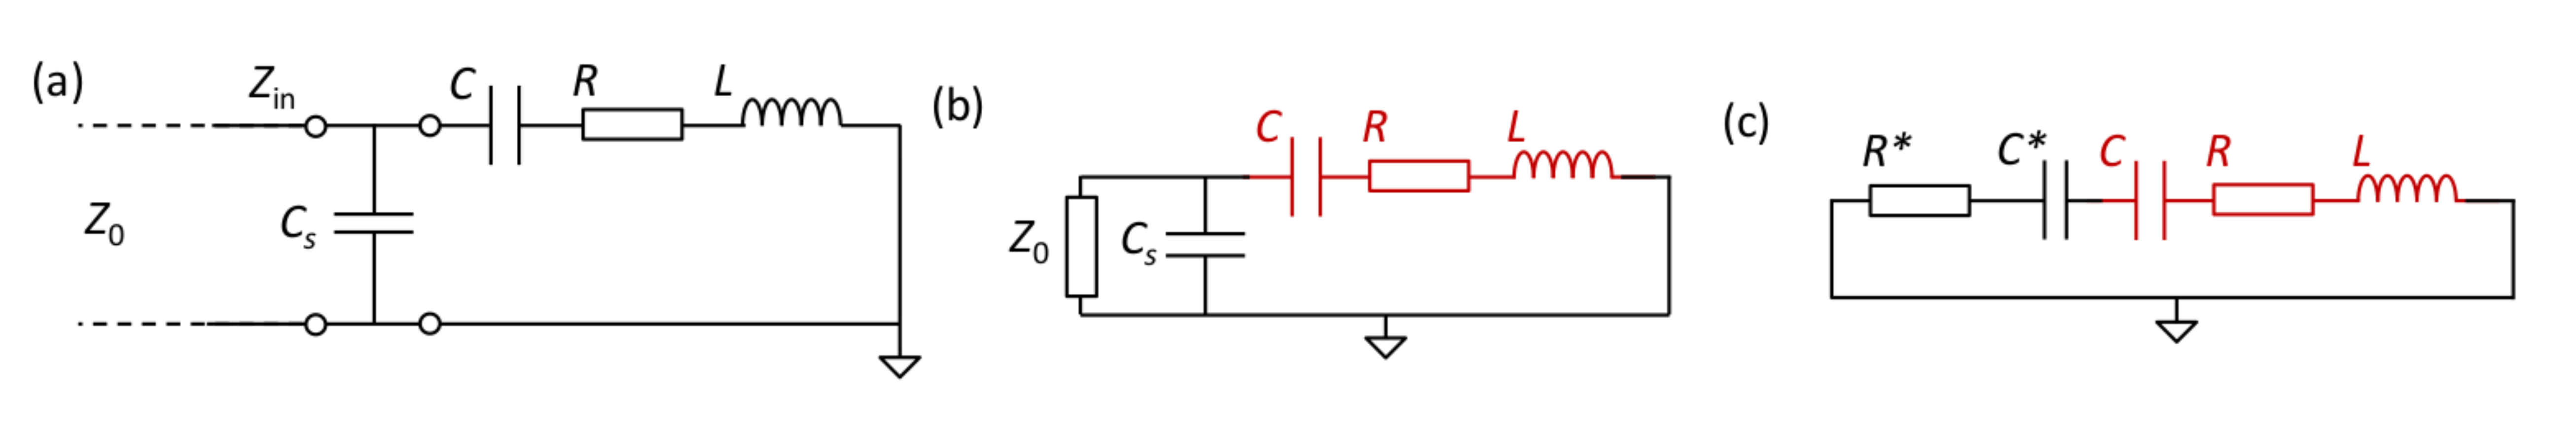
\includegraphics[width=0.7\linewidth]{chapter-theory/figs-RF/resonator_Daniel_crop}
	\caption{Lumped element model of a series RLC circuit capacitively coupled to one side of a transmission line. (a) Transmission line model. (b) Equivalent lumped element circuit. (c) Transformation to effective series circuit.}
	\label{fig:resonatordaniel}
\end{figure}

We analyze the circuit depicted in Fig. \ref{fig:resonatordaniel}. Typically we can assume $C_s\gg C$. The shunt capacitor and feedline have the total impedance
\begin{align}
Z_e = \left(\frac{1}{Z_0}+i\omega C_s\right)^{-1} = \frac{Z_0}{1+i\omega C_s} &= \frac{Z_0}{1+(\omega C_s Z_0)^2} + \frac{1}{i\omega}\frac{\omega^2 C_s Z_0^2}{1+(\omega C_s Z_0)^2} \\%
&= R^* + \frac{1}{i\omega}\frac{1}{C^*}
\end{align}
Hence we can transform the shunt capacitor and transmision line impedance into a series system together with the $RLC$-resonator. For this type of coupling, usually $\omega C_s Z_0\gg1$ aournd the resonance $\omega\approx\omega_0$. Hence, we can define these lumped elements as
\begin{align}
R^* \approx \frac{1}{\omega_0^2 C_s^2 Z_0}, \hspace{2cm}C^*\approx C_s
\end{align}
Then, for the total capacitance and resistance, we get 
\begin{align}
R_\mathrm{tot} = R+R^*, \hspace{2cm} C_\mathrm{tot}=\frac{C C_s}{C + C_s}
\end{align}

This lumped element circuit has the resonance frequency
\begin{align}
\omega_0 = \frac{1}{\sqrt{LC_\mathrm{tot}}} = \sqrt{\frac{C+C_s}{L C C_s}}
\end{align}
We can see that the coupling capacitor $C_s$ shifts the resonance frequency upwards, compared to the bare resonance frequency.
The total quality factor,
\begin{equation}
Q_L = \frac{1}{\omega_0 R_\mathrm{tot}C_\mathrm{tot}} = \left(\frac{1}{Q_\mathrm{int}} + \frac{1}{Q_\mathrm{ext}}\right)^{-1}
\end{equation}
can be separated into its internal and external components
\begin{align}
Q_\mathrm{int} &= \frac{C+C_s}{\omega_0 R C C_s}, \hspace{2cm} Q_\mathrm{ext} = \frac{C+C_s}{\omega_0 R^* C C_s} = \frac{\omega_0 Z_0 C_S (C+C_s)}{C} \\%
\kappa_\mathrm{ext} &= \frac{\omega_0}{Q_\mathrm{ext}} = \frac{\omega_0 R C C_s}{C+C_s}, \hspace{2cm} \kappa_\mathrm{ext} = \frac{\omega_0}{Q_\mathrm{ext}} = \frac{C}{Z_0 C_s (C+C_s)}
\end{align}
We can now calculate the complete input impedance of this circuit for the lossless case, i.e. $R=0$:
\begin{align}
\frac{1}{Z_\mathrm{in}}&=\left(i\omega L + \frac{1}{i\omega C}\right)^{-1} + i\omega C_s = i\frac{\omega(C+C_s)-\omega^3LCC_s}{1-\omega^2LC} \\%
&=i\omega\frac{C+C_s}{1-\omega^2LC}\left(1-\frac{\omega^2}{\omega_0^2}\right), \hspace{2cm} \omega_0=\frac{C+C_s}{LCC_s} \\%
&\approx2i\frac{C_s(C+C_s)}{C}\Delta\omega \\%
&\longrightarrow Z_\mathrm{in} \approx \frac{C}{C_s (C+C_s)}\frac{1}{\kappa_\mathrm{int}+2i\Delta\omega}.
\end{align}

With this, we get for the reflection parameter
\begin{equation}
\Gamma = \frac{Z_\mathrm{in}-Z_0}{Z_\mathrm{in}+Z_0}\approx\frac{\kappa_\mathrm{ext}-\kappa_\mathrm{int}-2i\Delta\omega}{\kappa_\mathrm{ext}+\kappa_\mathrm{int}+2i\Delta\omega}.
\end{equation}